\documentclass[tikz,border=4pt]{standalone}
\usepackage{helvet}
\renewcommand{\familydefault}{\sfdefault}
\usetikzlibrary{arrows.meta,positioning,fit,backgrounds}
\definecolor{blue}{HTML}{2A78D6}\definecolor{lblue}{HTML}{E4EEFA}
\definecolor{grey}{HTML}{898781}\definecolor{lgrey}{HTML}{F4F3EE}\definecolor{muted}{HTML}{52514E}
\definecolor{orange}{HTML}{EB6834}\definecolor{lorange}{HTML}{FCE9E1}
\begin{document}
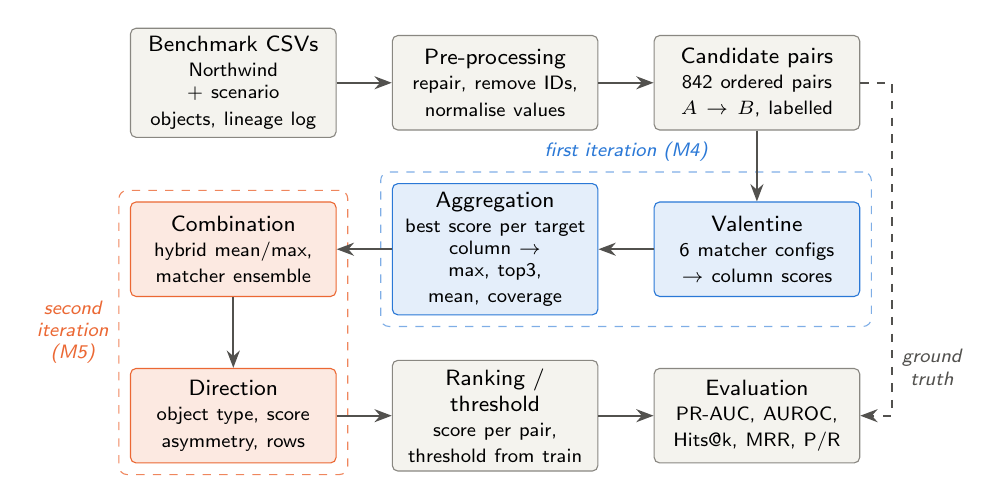
\begin{tikzpicture}[
  font=\footnotesize,
  box/.style={draw=grey, fill=lgrey, rounded corners=2pt, align=center, minimum height=12mm, text width=24mm, inner sep=3pt},
  core/.style={box, draw=blue, fill=lblue},
  new/.style={box, draw=orange, fill=lorange},
  arr/.style={-{Stealth[length=2.2mm]}, draw=muted, thick},
  lab/.style={font=\scriptsize\itshape, text=muted, align=center}]
\node[box] (csv) {Benchmark CSVs\\[1pt]\scriptsize Northwind + scenario\\objects, lineage log};
\node[box, right=7mm of csv] (pre) {Pre-processing\\[1pt]\scriptsize repair, remove IDs,\\normalise values};
\node[box, right=7mm of pre] (pairs) {Candidate pairs\\[1pt]\scriptsize 842 ordered pairs\\$A \rightarrow B$, labelled};
\node[core, below=9mm of pairs] (val) {Valentine\\[1pt]\scriptsize 6 matcher configs\\$\rightarrow$ column scores};
\node[core, left=7mm of val] (agg) {Aggregation\\[1pt]\scriptsize best score per target\\column $\rightarrow$ max, top3,\\mean, coverage};
\node[new, left=7mm of agg] (comb) {Combination\\[1pt]\scriptsize hybrid mean/max,\\matcher ensemble};
\node[new, below=9mm of comb] (dir) {Direction\\[1pt]\scriptsize object type, score\\asymmetry, rows};
\node[box, right=7mm of dir] (rank) {Ranking / threshold\\[1pt]\scriptsize score per pair,\\threshold from train};
\node[box, right=7mm of rank] (eval) {Evaluation\\[1pt]\scriptsize PR-AUC, AUROC,\\Hits@k, MRR, P/R};
\draw[arr] (csv) -- (pre); \draw[arr] (pre) -- (pairs); \draw[arr] (pairs) -- (val);
\draw[arr] (val) -- (agg); \draw[arr] (agg) -- (comb);
\draw[arr] (comb) -- (dir); \draw[arr] (dir) -- (rank); \draw[arr] (rank) -- (eval);
\draw[arr, dashed] (pairs.east) -| ++(4mm,-30mm) |- (eval.east) node[lab, pos=0.25, right]{ground\\truth};
\begin{scope}[on background layer]
\node[fit=(val)(agg), draw=blue!60, dashed, rounded corners=3pt, inner sep=4pt, label={[lab,text=blue]above:first iteration (M4)}] {};
\node[fit=(comb)(dir), draw=orange!80, dashed, rounded corners=3pt, inner sep=4pt, label={[lab,text=orange]left:second\\iteration\\(M5)}] {};
\end{scope}
\end{tikzpicture}
\end{document}
